
% !TeX root = ../report.tex
La première étape de réalisation de ce projet consiste au choix des différents composants le constituant. Il est en effet nécessaire de déterminer par exemple quel type de moteur sera utilisé d'utiliser la bonne approche théorique.
Il est important de noter que les critères de choix ne sont pas toujours issus directement du cahier des charges. Cependant, ils permettent une sélection objective des meilleurs composants.
Les composants soumis à ces choix sont les composants principaux suivants:

\begin{itemize}
    \item Moteurs
    \item Drivers Moteurs
    \item Microcontrôleur
    \item Capteur, \Gls{imu}
\end{itemize}


\section{Moteurs}

\subsection{Critères de choix}
\begin{table}[H]
    \centering
    \begin{tabular}{|c|l|}
        \hline
        \textbf{Critère} & \textbf{Justification} \\
        \hline
        Vitesse de rotation & Permet une réaction rapide pour la stabilisation du robot. \\
        \hline
        Précision du contrôle de vitesse & Assure un contrôle fin du balancement et de la stabilité. \\
        \hline
        Synchronisation des moteurs & Évite les rotations parasites du robot. \\
        \hline
        Consommation énergétique & Améliore l'autonomie du système embarqué sur batterie. \\
        \hline
        Système de contrôle simple & Réduit la complexité électronique et facilite l'implémentation. \\
        \hline
    \end{tabular}
    \caption{Critères moteurs}
    \label{tab:criteres_moteurs}
\end{table}
Ces critères de choix sont utilisés afin de mettre en concurrence trois types de moteurs distincts, décrits ci-dessous.
\subsection{Moteur DC}
\subsubsection{Vitesse de rotation}

La vitesse de rotation d'un moteur à courant continu (DC) dépend de sa conception mécanique, laquelle varie fortement selon les modèles.

Il existe des moteurs DC plus lents mais offrant un couple plus élevé. Par exemple, en recherchant \textit{« DC motors with gearbox »} sur Distrelec, on trouve une gamme de modèles dont la vitesse de rotation varie approximativement entre :

$$
\omega_{\text{mot}} \in [10, 20000] \ \text{tr/min}
$$

\subsubsection{Précision du contrôle de vitesse}

La vitesse d'un moteur DC peut être contrôlée à l'aide d'un signal PWM.

Cependant, la vitesse de rotation ne peut pas être déterminée avec une grande précision uniquement par PWM. En effet, les tolérances de fabrication entraînent des différences de comportement entre moteurs, ce qui implique une relation PWM $\rightarrow$ vitesse non parfaitement reproductible d'un moteur à l'autre.

\subsubsection{Synchronisation des moteurs}

En boucle ouverte (\textit{open-loop}), c'est-à-dire sans encodeur permettant de mesurer la position angulaire des moteurs, il est impossible d'assurer une synchronisation précise entre deux moteurs.

Une telle approche nécessiterait donc l'ajout d'encodeurs pour fermer la boucle de contrôle.

\subsubsection{Consommation énergétique}

La consommation énergétique de ce type de moteur dépend directement de la puissance mécanique délivrée. Ainsi, il n'est pas nécessaire de maintenir une alimentation constante pour conserver une position, contrairement à un moteur pas à pas.

On peut exprimer la puissance électrique par :

$$
p(t) = u(t)\, i(t)
$$

et le courant en fonction du couple :

$$
i(t) = \frac{T(t)}{k_t}
$$

La consommation d'un moteur DC est donc directement liée au couple qu'il fournit.

\subsubsection{Système de contrôle}

Le système de contrôle de ce type de moteur repose sur un pont en H, permettant de contrôler le sens de rotation.

La vitesse est régulée par un signal PWM en tension. La position du moteur peut être mesurée à l'aide d'un encodeur placé en sortie.

L'ensemble est généralement intégré dans une boucle de régulation de type \Gls{pid} afin d'assurer un contrôle précis de la vitesse et/ou de la position.
\subsubsection{Résultat Moteur DC}

\begin{table}[H]
    \centering
    \begin{tabular}{|l|c|}
        \hline
        \textbf{Critère} & \textbf{Note (/10)} \\
        \hline
        Vitesse de rotation & $8/10$\\
        \hline
        Précision du contrôle de vitesse & $5/10$ \\
        \hline
        Synchronisation des moteurs & $6/10$\\
        \hline
        Consommation énergétique & $9/10$\\
        \hline
        Système de contrôle simple & $5/10$\\
        \hline
    \end{tabular}
    \caption{Résultat Moteur DC}
    \label{tab:resultat_moteur_dc}
\end{table}

$$
\text{Note globale} = \frac{35}{50}
$$

\subsection{Moteur pas à pas}
Le moteur pas à pas est un type de moteur largement utilisé dans les systèmes nécessitant des déplacements angulaires extrêmement précis (CNC, impression 3D, plotters, etc.).

Ces moteurs fonctionnent selon un principe de déplacement par incréments (\textit{steps} ou pas).

\subsubsection{Vitesse de rotation}

La vitesse de rotation d'un moteur pas à pas n'est généralement pas son point fort. Elle dépend de sa capacité à enchaîner les pas.

D'après les données disponibles en ligne, la vitesse maximale des moteurs pas à pas varie approximativement entre :

$$
\omega_{\text{mot}} \in [600, 1200] \ \text{tr/min}
$$

Il est important de noter que le couple diminue lorsque la vitesse augmente.

\subsubsection{Précision du contrôle de vitesse}

Le contrôle des moteurs pas à pas s'effectue généralement en boucle ouverte (\textit{open-loop}). Cette technologie permet un positionnement angulaire très précis.

L'utilisation d'un driver avec micro-stepping permet de subdiviser chaque pas en micro-pas, améliorant encore la précision.

Par exemple, pour un moteur de 200 pas par tour avec un micro-stepping de 16, la résolution angulaire est :

$$
\theta = \frac{360^\circ}{200 \cdot 16} \approx 0.1125^\circ
$$

Cependant, comme le système est en boucle ouverte, aucune information de position réelle n'est disponible en sortie moteur. Il est donc difficile de détecter un décrochage (\textit{stall}).

Ainsi, si un pas est perdu, cette erreur n'est pas forcément détectée. Toutefois, en dimensionnant correctement le système (couple adapté à la charge), on peut limiter fortement ce risque.

\subsubsection{Synchronisation des moteurs}

La synchronisation entre deux moteurs pas à pas est généralement très bonne. En l'absence de décrochage, ils peuvent être considérés comme parfaitement synchrones.

\subsubsection{Consommation énergétique}

Le moteur pas à pas se distingue négativement sur ce point.

Afin de maintenir une position, il est nécessaire d'alimenter en permanence les bobines, ce qui entraîne une consommation énergétique élevée par rapport aux autres technologies.

\subsubsection{Système de contrôle}

Le contrôle d'un moteur pas à pas repose sur des drivers permettant de configurer le micro-stepping (généralement de 1 à 32 micro-pas par pas).

Le contrôle se fait via deux signaux principaux :

\begin{itemize}
    \item \textbf{STEP} : chaque impulsion correspond à un micro-pas
    \item \textbf{DIR} : définit le sens de rotation
\end{itemize}

\subsubsection{Synthèse des performances}

\begin{table}[H]
    \centering
    \begin{tabular}{|l|c|}
        \hline
        \textbf{Critère} & \textbf{Note (/10)} \\
        \hline
        Vitesse de rotation & 5/10 \\
        \hline
        Précision du contrôle de vitesse & 10/10 \\
        \hline
        Synchronisation des moteurs & 10/10 \\
        \hline
        Consommation énergétique & 3/10 \\
        \hline
        Système de contrôle & 7/10 \\
        \hline
    \end{tabular}
    \caption{Résultats Moteur Pas à pas}
    \label{tab:stepper_resultats}
\end{table}

$$
\text{Note globale} = \frac{35}{50}
$$

\subsection{Moteur Brushless}

Le moteur brushless est un type de moteur très efficace, présentant un excellent rapport couple/poids. Il permet d'atteindre des vitesses de rotation très élevées.

\subsubsection{Vitesse de rotation}

La vitesse de rotation d'un moteur brushless peut être très élevée.

En cherchant sur internet différents modèles, on trouve des vitesses maximales variant entre:

$$
\omega_{\text{mot}} \in [10\,000, 50\,000] \ \text{tr/min}
$$

Il s'agit donc d'un moteur extrêmement rapide et réactif.

Cependant, il est plus difficile d'obtenir un contrôle précis à basse vitesse, ce qui est critique pour ce projet, car le robot doit pouvoir effectuer de très faibles variations de vitesse afin de maintenir son équilibre.

\subsubsection{Précision du contrôle de vitesse}

Le contrôle des moteurs brushless peut être réalisé selon deux approches principales.

La première utilise des capteurs à effet Hall permettant de déterminer la position du rotor et de commander les phases au bon moment.

La seconde repose sur la mesure de la force contre-électromotrice (\textit{Back-EMF}) dans les phases non alimentées afin d'estimer la position du rotor.

Une fois la position connue, plusieurs méthodes de commande sont possibles :

\paragraph{Commande trapézoïdale}
Cette méthode consiste à alimenter deux des trois phases simultanément.

Elle est simple à implémenter, mais génère des variations brusques de couple et est peu performante à basse vitesse.

\paragraph{\Gls{foc}}
La commande \Gls{foc} repose sur la décomposition du courant moteur en deux composantes orthogonales via les transformations de Clarke et Park.

Cette méthode permet :
\begin{itemize}
    \item un mouvement fluide,
    \item une meilleure efficacité énergétique,
    \item un excellent contrôle à basse vitesse.
\end{itemize}

Dans le cadre de ce projet, une commande trapézoïdale seule n'est pas suffisante et doit idéalement être remplacée par une commande FOC.

\subsubsection{Synchronisation des moteurs}

La synchronisation dépend fortement de la qualité de l'ESC (Electronic Speed Controller).

Avec une commande FOC, il est possible d'obtenir une bonne synchronisation des vitesses entre moteurs.

\subsubsection{Consommation énergétique}

La consommation d'un moteur brushless dépend du couple fourni.

Cependant, contrairement au moteur DC, l'électronique de commande (ESC) consomme également de l'énergie, ce qui doit être pris en compte dans le bilan global.

\subsubsection{Système de contrôle}

Le contrôle d'un moteur brushless nécessite un ESC (Electronic Speed Controller).

Pour obtenir de bonnes performances, il est nécessaire d'avoir une estimation de la position du rotor.

Cependant, la détection par Back-EMF est peu efficace à basse vitesse, ce qui rend la commande complexe et coûteuse à mettre en oeuvre.

\subsubsection{Synthèse des performances}

\begin{table}[H]
    \centering
    \begin{tabular}{|l|c|}
        \hline
        \textbf{Critère} & \textbf{Note (/10)} \\
        \hline
        Vitesse de rotation & 7/10 \\
        \hline
        Précision du contrôle de vitesse & 8/10 \\
        \hline
        Synchronisation des moteurs & 8/10 \\
        \hline
        Consommation énergétique & 4/10 \\
        \hline
        Système de contrôle & 1/10 \\
        \hline
    \end{tabular}
    \caption{Synthèse des performances du moteur brushless}
    \label{tab:brushless_resultats}
\end{table}

$$
\text{Note globale} = \frac{28}{50}
$$

\subsection{Choix final}
À l'issue de l'analyse des trois technologies étudiées (moteur DC, moteur pas à pas et moteur brushless), le moteur pas à pas apparaît comme le meilleur compromis pour ce projet.

Bien qu'il présente une consommation énergétique plus élevée que les autres solutions et une vitesse maximale plus limitée, il se distingue clairement sur les critères essentiels au bon fonctionnement du système.

En effet, le moteur pas à pas offre :

\begin{itemize}
    \item une excellente précision de contrôle grâce au micro-stepping,
    \item une très bonne synchronisation entre moteurs en fonctionnement normal,
    \item un contrôle simple basé sur des signaux STEP/DIR,
    \item une bonne répétabilité du mouvement en boucle ouverte.
\end{itemize}

Ces caractéristiques sont particulièrement adaptées à un système de stabilisation, où la précision des petits déplacements et la synchronisation des moteurs sont des éléments critiques.

De plus, la simplicité de mise en oeuvre des drivers pas à pas permet de limiter la complexité électronique globale du système, ce qui constitue un avantage important dans le cadre de ce projet embarqué.

Ainsi, malgré ses limites en termes de rendement énergétique et de vitesse maximale, le moteur pas à pas est retenu comme solution finale, car il répond le mieux aux exigences de précision, de contrôle et de simplicité imposées par le cahier des charges.

\section{Drivers moteurs}
\subsection{Critères de choix}
\begin{table}[H]
    \centering
    \begin{tabular}{|c|l|}
        \hline
        \textbf{Critère} & \textbf{Justification} \\
        \hline
        Microstepping & Permet un réglage fin de la vitesse des moteurs. \\
        \hline
        Taille & Étant donné la nature embarquée du système, la taille des modules est un critère important. \\
        \hline
        Efficacité énergétique & Le système fonctionnant sur batterie, les modules doivent dissiper le moins d'énergie possible. \\
        \hline
        Bruit & Les drivers doivent être silencieux en fonctionnement. \\
        \hline
    \end{tabular}
    \caption{Critères de sélection des drivers moteurs}
    \label{tab:criteres_drivers}
\end{table}

\subsection{A4988}

Le A4988 \cite{A4988_datasheet} est un driver de moteur pas à pas couramment utilisé pour des applications embarquées.

\subsubsection{Tensions de fonctionnement}

\begin{itemize}
    \item Tension moteur : $V_{\mathrm{mot}} \in [8, 35]\,\mathrm{V}$
    \item Tension logique : $V_{\mathrm{DD}} \in [3, 5.5]\,\mathrm{V}$
\end{itemize}

\subsubsection{Microstepping}

Le module propose un système de micro-pas permettant les subdivisions suivantes :
$$
1,\; \frac{1}{2},\; \frac{1}{4},\; \frac{1}{8},\; \frac{1}{16} \;\; \mu\mathrm{step/step}
$$

\subsubsection{Taille}

Environ $20 \times 15\,\mathrm{mm}$.

\subsubsection{Consommation}

Il est difficile d'estimer précisément la consommation moyenne de ce module, celle-ci dépendant fortement du mode de fonctionnement et de la charge moteur.

Cependant, le A4988 est un driver simple, peu sophistiqué et peu coûteux, mais dont le rendement énergétique reste limité.

\subsubsection{Bruit}

Le A4988 peut générer un bruit audible relativement important, en particulier à courant élevé et en l'absence d'optimisation du microstepping.

\begin{table}[H]
    \centering
    \begin{tabular}{|l|c|}
        \hline
        \textbf{Critère} & \textbf{Note (/10)} \\
        \hline
        Tension de fonctionnement & 9/10 \\
        \hline
        Microstepping & 6/10 \\
        \hline
        Consommation & 4/10 \\
        \hline
        Bruit & 3/10 \\
        \hline
    \end{tabular}
    \caption{Résultats critères A4988}
    \label{tab:a4988_resultats}
\end{table}

$$
\text{Note globale} = \frac{22}{50}
$$

\subsection{TMC2226}

Le TMC2226 \cite{TMC2226_datasheet} est un driver de moteur pas à pas développé par Trinamic, destiné aux applications embarquées nécessitant un fonctionnement silencieux et une bonne efficacité énergétique.

Contrairement à des drivers plus simples tels que le A4988, le TMC2226 intègre des fonctionnalités avancées de contrôle de courant, permettant une réduction significative du bruit acoustique du moteur, ainsi qu'une gestion de consommation. Il propose également des modes de microstepping très fins, améliorant la fluidité et la précision du mouvement.
Ce dernier est paramètrable via une pin \Gls{uart} bidirectionnelle.

\subsubsection{Tensions de fonctionnement}

\begin{itemize}
    \item Tension moteur : $V_{\mathrm{mot}} \in [5.5, 29]\,\mathrm{V}$
    \item Tension logique : $V_{\mathrm{DD}} \in [3.3, 5]\,\mathrm{V}$
\end{itemize}

\subsubsection{Microstepping}

Le TMC2226 supporte un microstepping très élevé avec interpolation interne, permettant d'atteindre une résolution jusqu'à :
$$
1,\; \frac{1}{2},\; \frac{1}{4},\; \frac{1}{8},\; \frac{1}{16},\; \frac{1}{32},\; \frac{1}{64},\; \frac{1}{128},\; \frac{1}{256}
$$

\subsubsection{Taille}

Environ $9.7 \times 6.4\,\mathrm{mm}$ pour le circuit intégré (selon encapsulation), ou variable selon les modules d'évaluation.

\subsubsection{Consommation}

La consommation du TMC2226 dépend fortement du courant moteur configuré et du mode de fonctionnement.

Grâce à ses algorithmes de contrôle avancés, il permet une optimisation de la consommation énergétique, notamment en charge partielle ou à faible vitesse.

\subsubsection{Bruit}

Le TMC2226 est conçu pour fonctionner de manière très silencieuse, réduisant fortement les vibrations et les nuisances acoustiques, même à bas régime.
\begin{table}[H]
    \centering
    \begin{tabular}{|l|c|}
        \hline
        \textbf{Critère} & \textbf{Note (/10)} \\
        \hline
        Tension de fonctionnement & 8/10 \\
        \hline
        Microstepping & 10/10 \\
        \hline
        Consommation & 9/10 \\
        \hline
        Bruit & 10/10 \\
        \hline
    \end{tabular}
    \caption{Résultats critères TMC2226}
    \label{tab:tmc2226_resultats}
\end{table}

$$
\text{Note globale} = \frac{37}{50}
$$


\subsection{Choix final}

À l'issue de l'analyse des deux drivers étudiés (A4988 et TMC2226), le TMC2226 apparaît comme la solution la plus adaptée aux besoins du projet.

Bien que son coût soit supérieur à celui du A4988 et que sa configuration puisse être légèrement plus complexe, il offre des performances nettement supérieures sur les critères essentiels au bon fonctionnement du système.

En effet, le TMC2226 se distingue par :

\begin{itemize}
    \item un microstepping jusqu'à $\frac{1}{256}$ avec interpolation interne, offrant un mouvement particulièrement fluide et précis ;
    \item une consommation énergétique optimisée grâce à sa gestion avancée du courant ;
    \item un fonctionnement très silencieux, réduisant fortement les vibrations et le bruit acoustique ;
    \item une interface de contrôle compatible STEP/DIR ainsi qu'une configuration via \Gls{uart}, permettant un réglage fin des paramètres du driver.
\end{itemize}

Ces caractéristiques sont particulièrement adaptées à un système de stabilisation embarqué, où la précision des mouvements, la réduction des vibrations et l'autonomie énergétique sont des critères déterminants.

De plus, malgré une mise en œuvre légèrement plus avancée que celle de l'A4988, le TMC2226 reste simple à intégrer tout en apportant des fonctionnalités supplémentaires qui améliorent les performances globales du système.

Ainsi, le TMC2226 est retenu comme driver moteur pour ce projet, car il répond le mieux aux exigences de précision, de silence de fonctionnement et d'efficacité énergétique imposées par le cahier des charges.

\section{Microcontrôleur}
\subsection{Critères de choix}
\begin{table}[H]
    \centering
    \begin{tabular}{|c|l|}
        \hline
        \textbf{Critère} & \textbf{Justification} \\
        \hline
        Fréquence de travail & Nécessaire afin de réguler rapidement le système, ainsi que d'offrir une interface de contrôle \\
        \hline
        Taille & Comme cité pour le reste des composants, la taille ne doit pas être trop importante. \\
        \hline
        Efficacité énergétique & Le module ne dois pas être trop gourmand en énergie. \\
        \hline
        Communication sans fil & Afin de pouvoir contrôler le système à distance, le contrôleur doit offrir une capacité de communication sans fil \\
        \hline
    \end{tabular}
    \caption{Critères de sélection du microcontrôleur}
    \label{tab:criteres_microcontroleur}
\end{table}
\subsection{ESP-32 DevKit V1}

L'ESP-32 DevKit V1 \cite{ESP-32-Devkit-V1} est une carte de développement intégrant, comme son nom l'indique, un microcontrôleur de type ESP-32 \cite{ESP-32_Series}. 

Cette carte de développement met à disposition 21 entrées/sorties (\acrshort{gpio}), ce qui la rend particulièrement adaptée aux applications embarquées.

L'ESP-32 inclut également une antenne \acrshort{pcb}, permettant une communication sans fil via WiFi ou Bluetooth.

\subsubsection{Fréquence de travail}

L'ESP-32 peut fonctionner jusqu'à une fréquence d'horloge maximale de $240\,\si{\mega\hertz}$.

\subsubsection{Taille}

Les dimensions du module ESP-32 DevKit V1 sont présentées ci-dessous :

\begin{figure}[H]
    \centering
    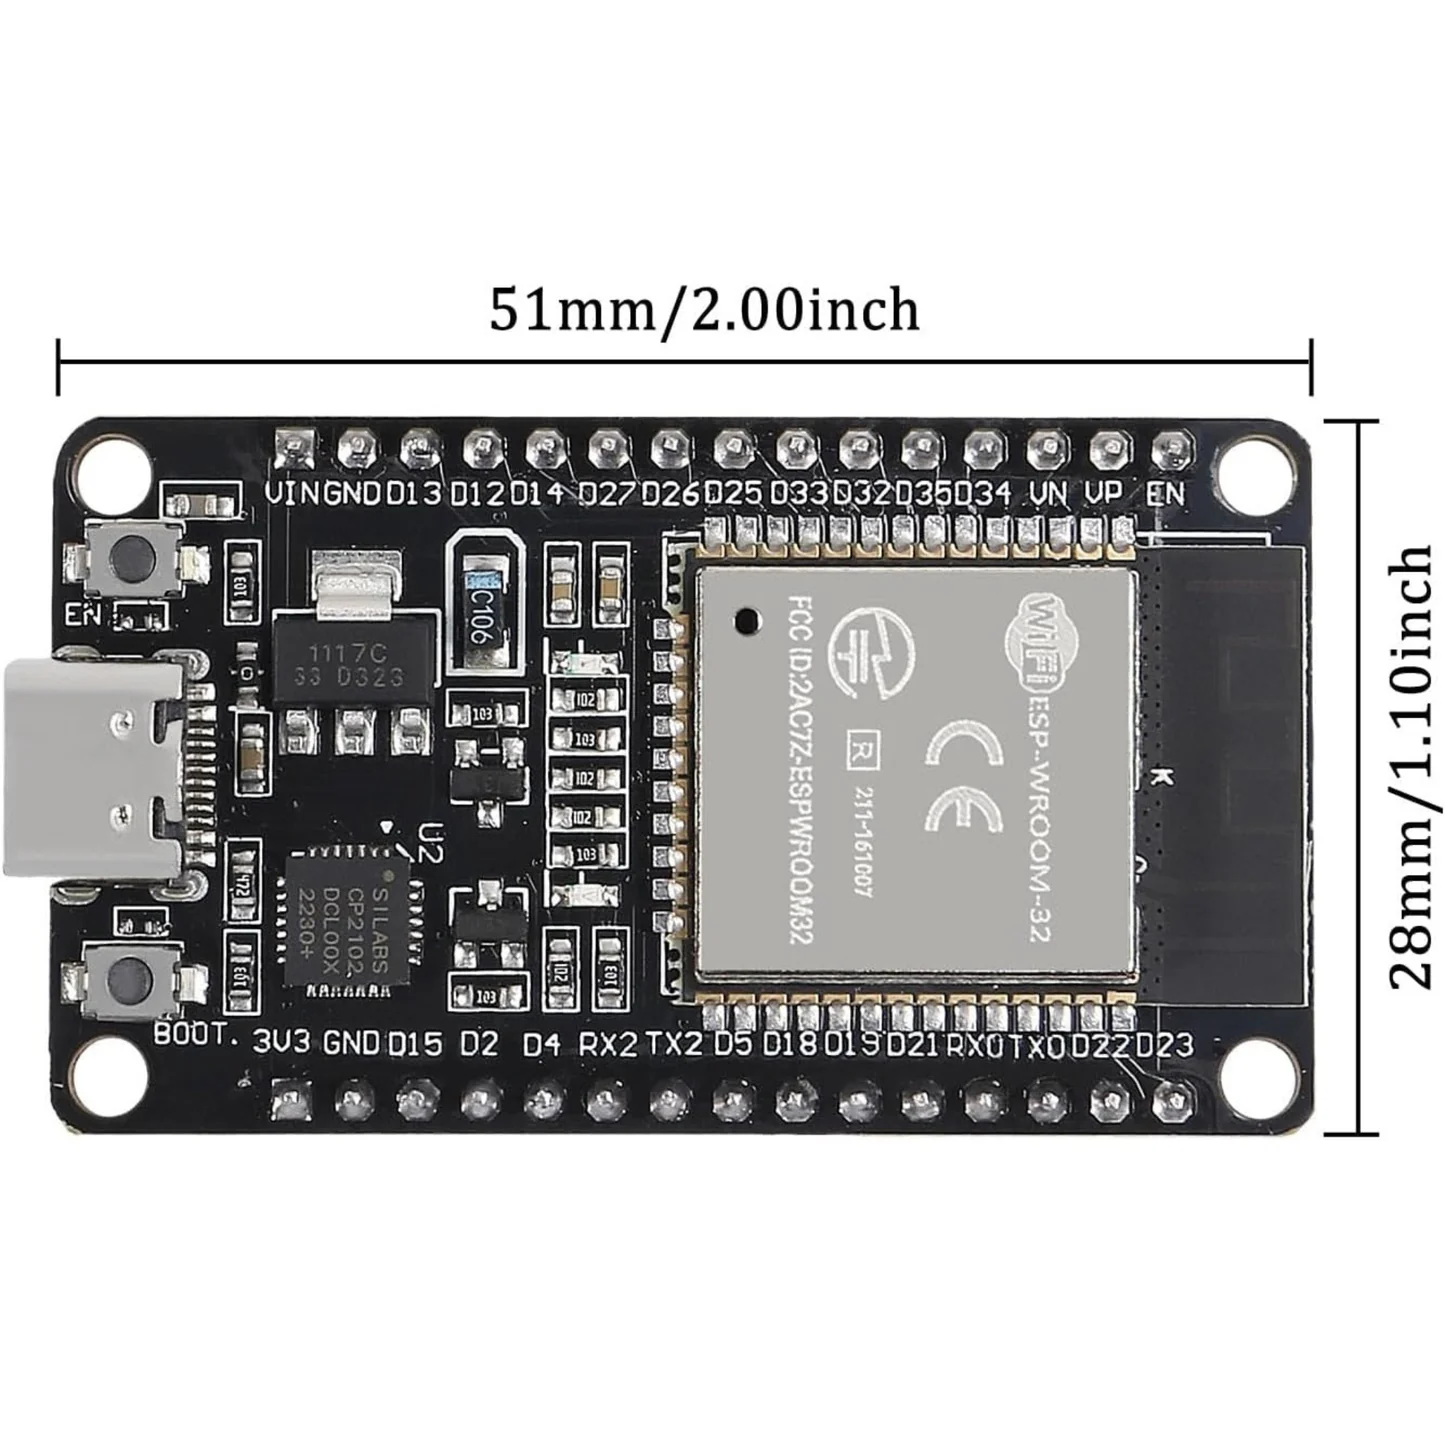
\includegraphics[width=0.6\textwidth]{assets/figures/esp32_devkit_v1.png}
    \caption{Dimensions du module ESP-32 DevKit V1}
    \label{fig:esp32_dimensions}
\end{figure}

\subsubsection{Efficacité énergétique}

D'après le datasheet de l'ESP-32, sa consommation électrique dépend fortement du mode de fonctionnement (veille, WiFi actif, Bluetooth actif, etc.).

\begin{figure}[H]
    \centering
    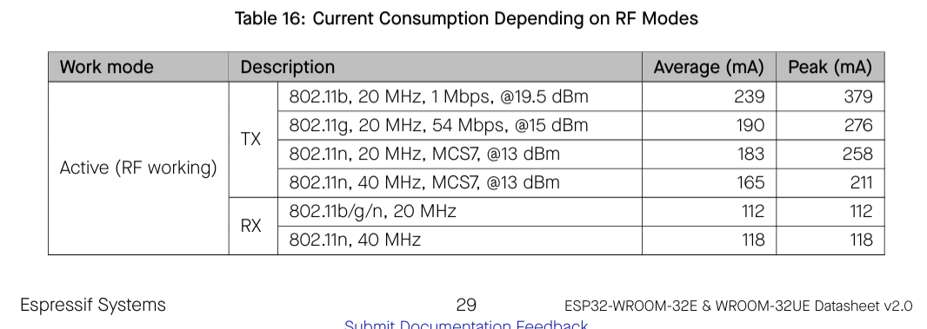
\includegraphics[width=0.75\textwidth]{assets/figures/esp32_consumption.png}
    \caption{Consommation énergétique de l'ESP-32 selon le mode de fonctionnement}
    \label{fig:esp32_power}
\end{figure}

\subsubsection{Communication sans fil}

Comme indiqué précédemment, l'ESP-32 inclut une antenne intégrée permettant la communication sans fil via WiFi et Bluetooth, offrant ainsi une grande flexibilité pour les applications connectées.

\begin{table}[H]
    \centering
    \begin{tabular}{|l|c|}
        \hline
        \textbf{Critère} & \textbf{Note (/10)} \\
        \hline
        Fréquence de travail & 9/10 \\
        \hline
        Taille & 7/10 \\
        \hline
        Efficacité énergétique & 7/10 \\
        \hline
        Communication sans fil & 8/10\\
        \hline
    \end{tabular}
    \caption{Résultats critères ESP-32 Devkit V1}
    \label{tab:esp32_results}
\end{table}

$$
\text{Note globale} = \frac{31}{50}
$$
\subsection{Raspberry Pi Pico W}

Le Raspberry Pi Pico W \cite{RaspberryPiPicoW} est une carte de développement basée sur le microcontrôleur RP2040, développée par la fondation Raspberry Pi. Il s'agit d'une évolution du Raspberry Pi Pico, à laquelle a été ajouté un module de communication sans fil.

Contrairement à des cartes plus complètes comme l'ESP-32 DevKit V1 \cite{ESP-32-Devkit-V1}, le Pico W ne dispose pas de Bluetooth, mais intègre une connectivité WiFi 2.4 GHz.

Cette carte peut être programmée en C/C++ via le SDK officiel, ainsi qu'en MicroPython, ce qui la rend accessible aussi bien pour le prototypage que pour des applications embarquées avancées.

\subsubsection{Fréquence de travail}

Le Raspberry Pi Pico W fonctionne jusqu'à une fréquence d'horloge de $133\,\si{\mega\hertz}$ grâce à son processeur double cœur ARM Cortex-M0+.

\subsubsection{Taille}

Les dimensions du module Raspberry Pi Pico W sont compactes, ce qui facilite son intégration dans des systèmes embarqués :

\begin{figure}[H]
    \centering
    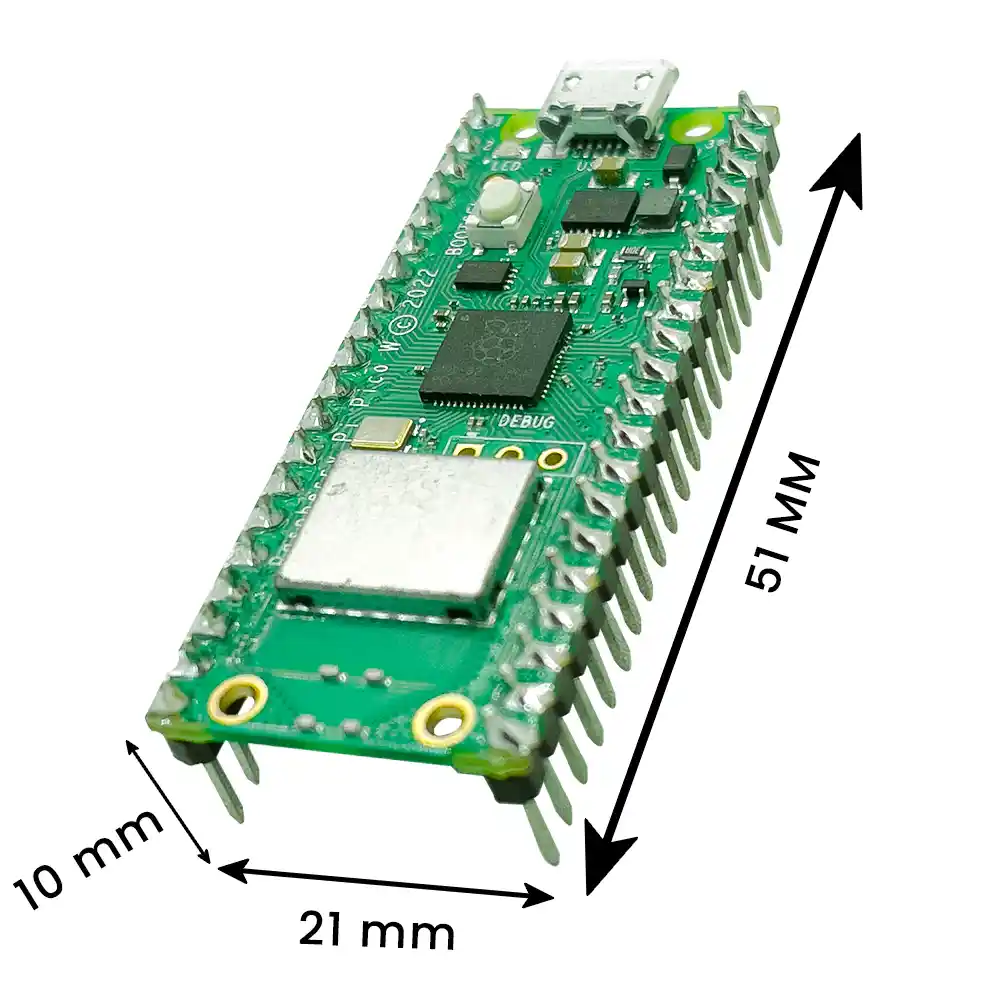
\includegraphics[width=0.6\textwidth]{assets/figures/raspberry_pico_w_dimensions.png}
    \caption{Dimensions du Raspberry Pi Pico W}
    \label{fig:pico_w_dimensions}
\end{figure}

\subsubsection{Efficacité énergétique}
Il est impossible de trouver avec précision une information relative à la consommation exacte de courant du module Raspberry Pico W. Cependant, en cherchant en ligne, voici ce que l'on peut trouver \href{https://stfn.pl/blog/34-pico-power-consumption-solar-panels/}{Raspberry Pico W Power consumption}.
Dans cette article, l'auteur décrit avoir observé un courant "continu" de $$0.45 \si\ampere$$ en ayant le wifi actif. Il ne s'agit bien entendu pas d'une mesure officielle du fabricant et il est donc nécessaire de la considérer avec suffisamment de recul.


\subsubsection{Communication sans fil}
Le Raspberry Pi Pico W intègre un module WiFi 2.4 GHz permettant la communication réseau. Toutefois, il ne supporte pas le Bluetooth, contrairement à certaines solutions concurrentes comme l'ESP32.

\begin{table}[H]
    \centering
    \begin{tabular}{|l|c|}
        \hline
        \textbf{Critère} & \textbf{Note (/10)} \\
        \hline
        Fréquence de travail & 7/10 \\
        \hline
        Taille & 9/10 \\
        \hline
        Efficacité énergétique & 8/10 \\
        \hline
        Communication sans fil & 6/10 \\
        \hline
    \end{tabular}
    \caption{Résultats critères Raspberry Pi Pico W}
    \label{tab:pico_results}
\end{table}

$$
\text{Note globale} = \frac{30}{50}
$$

\subsection{Choix final}

À l'issue de l'analyse comparative des deux microcontrôleurs étudiés (ESP-32 DevKit V1 et Raspberry Pi Pico W), le choix s'oriente vers l'ESP-32 DevKit V1.

Bien que le Raspberry Pi Pico W présente une meilleure efficacité énergetique et une taille inférieure à l'ESP, il reste limité par l'absence de Bluetooth ainsi que la fréquence d'horloge.

L'ESP-32 DevKit V1 se distingue par une meilleure polyvalence, notamment grâce à la présence du WiFi et du Bluetooth, une fréquence de travail plus élevée.


\section{IMU}
\subsection{Critères de choix}
\begin{table}[H]
    \centering
    \begin{tabular}{|c|l|}
        \hline
        \textbf{Critère} & \textbf{Justification} \\
        \hline
        Vitesse de lecture & Une lecture rapide des données permet une boucle de régulation plus rapide \\
        \hline
        Qualité du signal & Un signal bruité peut causer des problèmes dans la régulation \\
        \hline
        Taille & Comme le reste des composants, la taille du capteur doit être minimisée \\
        \hline
        Facilitée d'implémentation & Le capteur ne doit pas nécessiter des heures de travail d'implémentation\\
        \hline
        Prix & Le coût du capteur doit rester faible afin de limiter le coût total du robot. \\
        \hline
    \end{tabular}
    \caption{Critères de sélection de l'IMU}
    \label{tab:criteres_IMU}
\end{table}
\subsection{MPU6050}
Le premier candidat est le MPU6050, plus précisement la carte de développement GY-521 \cite{GY521_Datasheet}.
\subsubsection{Vitesse de lecture}
Les vitesse de lectures se trouvent dans le datasheet aux pages 12 et 13.
\begin{itemize}
    \item Fréquence max de lecture accéléromètre: 1 kHz;
    \item Fréquence max de lecture gyroscope:  8 kHz;
\end{itemize}
Les données sont accessibles via une interface I\textsuperscript{2}C simple à mettre en oeuvre \cite{MPU6050_Datasheet}.


\subsubsection{Qualité du signal}
Le capteur intègre un accéléromètre 3 axes et un gyroscope 3 axes 16 bits. 
Bien que plus ancien que les IMU récentes, il offre une qualité de mesure suffisante pour une estimation fiable de l'angle après application d'un filtre complémentaire software. Il n'intègre cependant pas de
filtrage de données embarqué.

\subsubsection{Taille}

\begin{figure}[H]
    \centering
    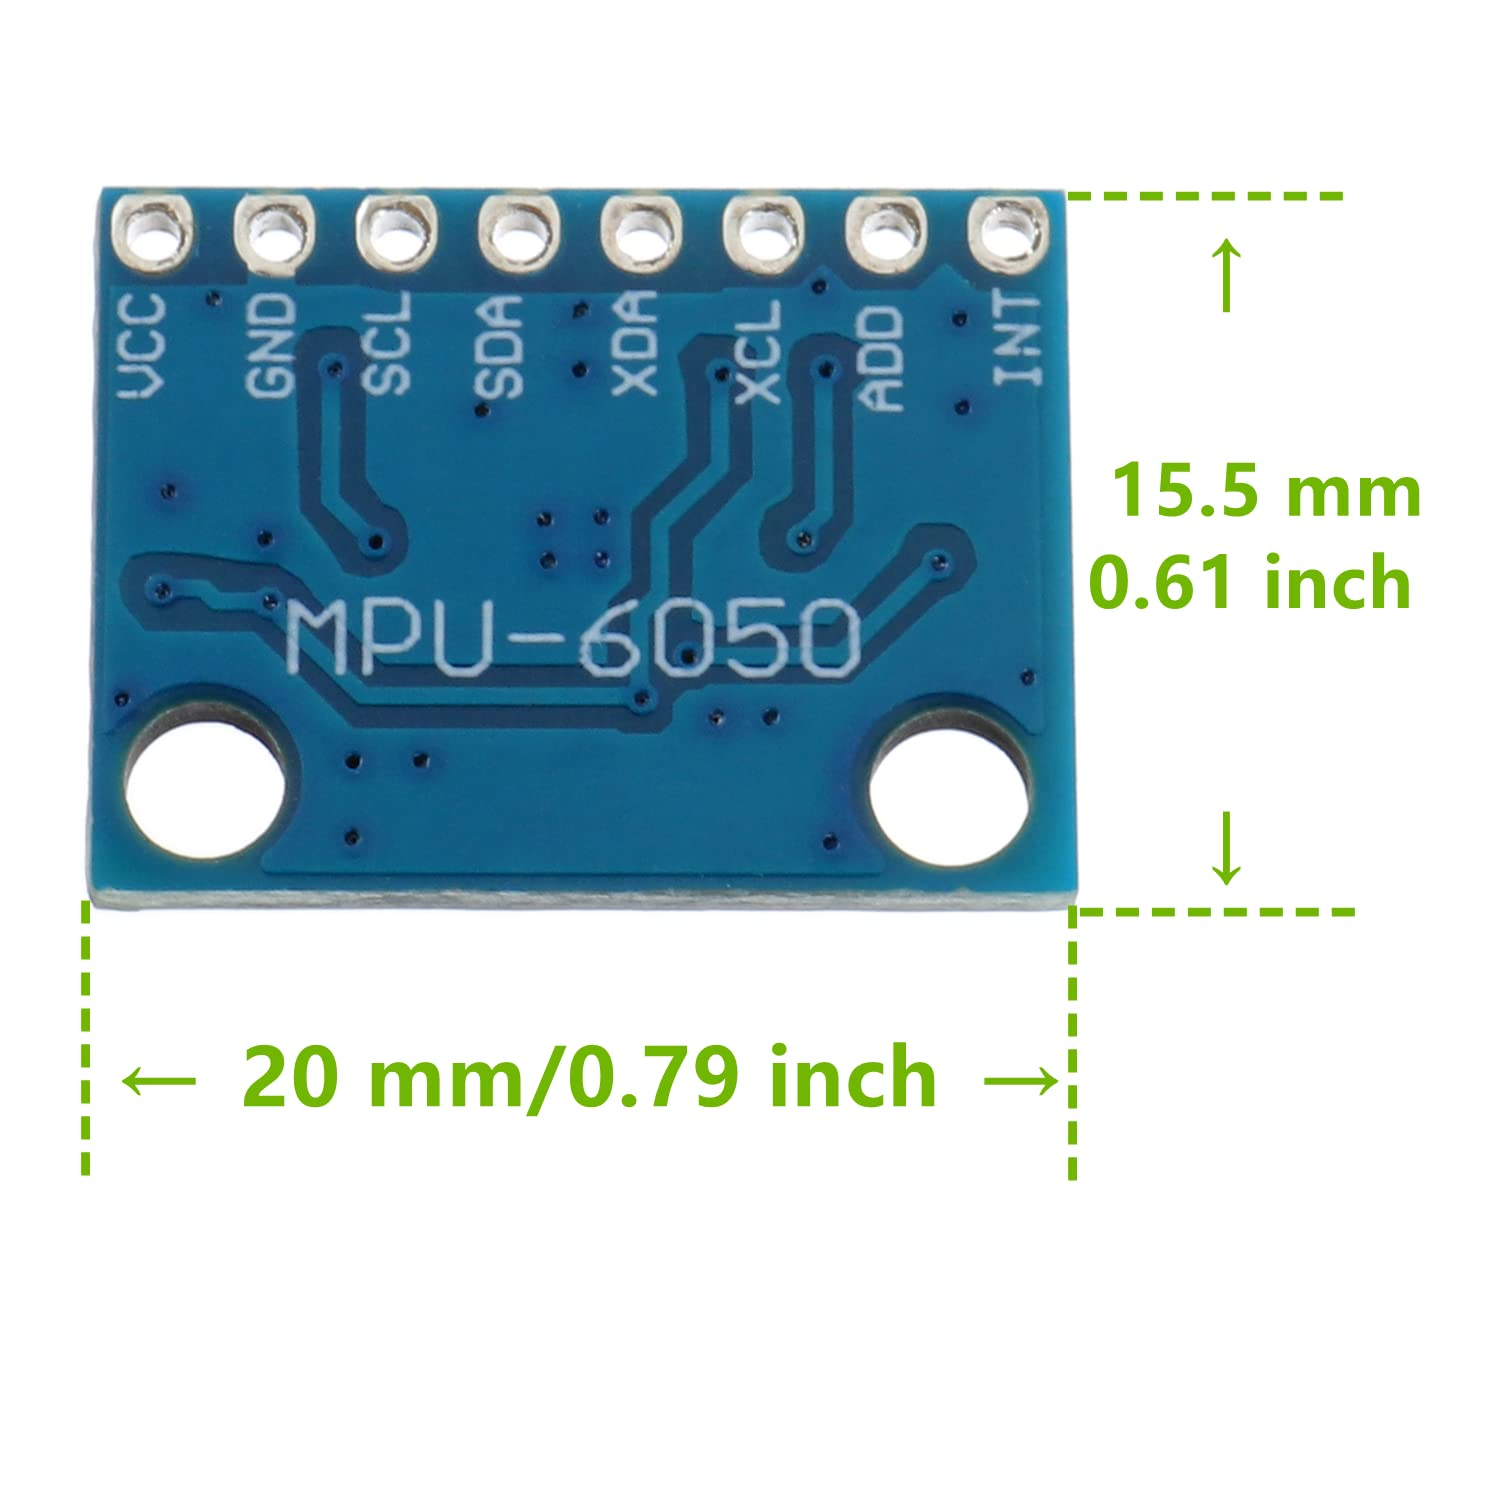
\includegraphics[width=0.6\textwidth]{assets/figures/mpu6050_dimensions.png}
    \caption{Dimensions de la carte GY-521}
    \label{fig:mpu_6050_dimensions}
\end{figure}


\subsubsection{Facilité d'implémentation}
Le MPU6050 est probablement l'IMU la plus documentée. De nombreuses bibliothèques Arduino et ESP-IDF existent, ce qui réduit fortement le temps de développement. 

\subsubsection{Prix}
Le module GY-521 basé sur le MPU6050 est très répandu et disponible chez de nombreux fournisseurs pour un prix compris entre 3 et 5 CHF. 
Son faible coût en fait une solution particulièrement intéressante pour les projets étudiants et les prototypes.
\begin{table}[H]
    \centering
    \begin{tabular}{|l|c|}
        \hline
        \textbf{Critère} & \textbf{Note (/10)} \\
        \hline
        Vitesse de lecture & 9/10 \\
        \hline
        Qualité du signal & 8/10 \\
        \hline
        Taille & 8/10 \\
        \hline
        Facilité d'implémentation & 10/10 \\
        \hline
        Prix & 10/10 \\
        \hline
    \end{tabular}
    \caption{Évaluation du MPU6050}
    \label{tab:mpu6050_resultats}
\end{table}

$$
\text{Note globale}=\frac{45}{50}
$$


\subsection{BMI160}

Le deuxième candidat est le BMI160, de chez Bosch.
\subsubsection{Vitesse de lecture}
Le BMI160 peut être paramétré afin d'offrir des fréquences de lectures variant de la manière suivante:
\begin{itemize}
    \item Gamme de fréquence de lecture accéléromètre: 12.5-1600 Hz;
    \item Gamme de fréquence de lecture gyroscope: 25-3200 Hz;
\end{itemize}
Le paramètrage se fait à l'aide des registres.

\subsubsection{Qualité du signal}
Grâce à une électronique plus récente, le BMI160 présente un bruit de mesure plus faible et une meilleure stabilité thermique que le MPU6050. 
Les mesures obtenues sont généralement plus précises.

\subsubsection{Taille}
\begin{figure}[H]
    \centering
    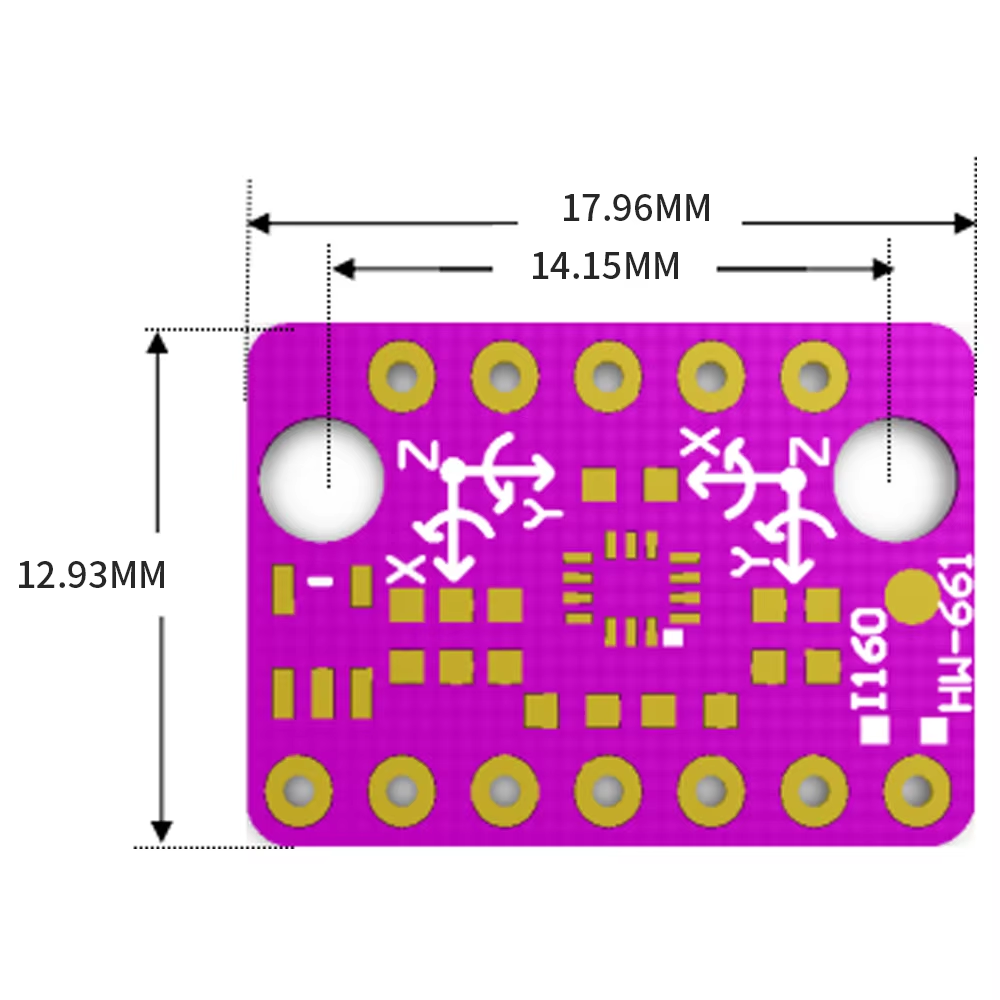
\includegraphics[width=0.6\textwidth]{assets/figures/bmi_160_dimensions.png}
    \caption{Dimensions du BMI160}
    \label{fig:bmi_160_dimensions}
\end{figure}

\subsubsection{Facilité d'implémentation}
Bien que plusieurs bibliothèques soient disponibles, le BMI160 nécessite une configuration plus complexe que le MPU6050. 
La documentation est également moins abondante au sein de la communauté des makers.

\subsubsection{Prix}

Les cartes de développement basées sur le BMI160 sont généralement vendues entre 6 et 10 CHF, soit environ deux fois plus cher qu'un module GY-521 intégrant le MPU6050.
\begin{table}[H]
    \centering
    \begin{tabular}{|l|c|}
        \hline
        \textbf{Critère} & \textbf{Note (/10)} \\
        \hline
        Vitesse de lecture & 10/10 \\
        \hline
        Qualité du signal & 9/10 \\
        \hline
        Taille & 9/10 \\
        \hline
        Facilité d'implémentation & 7/10 \\
        \hline
        Prix & 6/10 \\
        \hline
    \end{tabular}
    \caption{Évaluation du BMI160}
    \label{tab:bmi160_resultats}
\end{table}

$$
\text{Note globale}=\frac{41}{50}
$$
\subsection{Choix final}

Le BMI160 présente de meilleures performances en termes de qualité du signal et bénéficie d'une électronique plus récente. En revanche, ces avantages ne sont pas indispensables dans le cadre d'un robot auto-équilibré. Les performances du MPU6050 sont largement suffisantes pour atteindre la fréquence d'échantillonnage nécessaire et réaliser une estimation fiable de l'angle à l'aide d'un filtre logiciel.

Par ailleurs, le module GY-521 intégrant le MPU6050 est environ deux fois moins cher qu'une carte de développement basée sur le BMI160. Le grand nombre de bibliothèques disponibles et son faible coût permettent également de réduire le temps de développement ainsi que le coût global du projet.

Le choix s'est donc porté sur le \textbf{MPU6050}, qui offre le meilleur compromis entre performances, simplicité d'intégration et coût pour cette application.